\chapter{Architettura software}\label{ch-04}

\lecturemeta{Capitolo originale: 4 --- Software Architecture \quad\textbullet\quad Antonio Brogi}{Appunti di Emiliano Sescu (github.com/Faxatos), cap. 4}

\begin{boxdefinition}{Architettura software}

L'\textbf{architettura} è l'organizzazione fondamentale di un sistema
software: i suoi \textbf{componenti}, le loro relazioni tra loro e con
l'ambiente, e i principi che ne guidano il design.

\end{boxdefinition}

L'architettura influenza prestazioni, usabilità, sicurezza,
affidabilità, manutenibilità e così via. È fatta di \textbf{componenti},
dove ogni componente implementa un insieme coerente di funzionalità
(\textbf{servizi} che altri componenti possono usare). Ecco un esempio
di come si usano i componenti:

\begin{figure}[H]
\centering
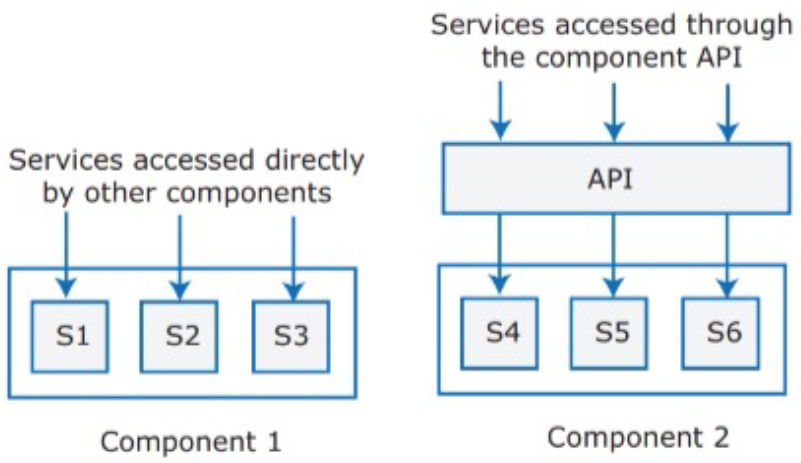
\includegraphics[width=0.70\linewidth,height=0.45\textheight,keepaspectratio]{images/04-architettura_fig4-1_api-componenti.png}
\caption{Chiamare i servizi di un componente tramite API.}
\end{figure}

Quando il software è grande bisogna sviluppare delle \textbf{API}
(\emph{Application Programming Interface}) per far comunicare i
componenti, che potrebbero anche essere realizzati con tecnologie
diverse.

Nel progettare il software si tengono in considerazione diversi aspetti:

\begin{itemize}
\tightlist
\item
  \textbf{Caratteristiche non funzionali}: sicurezza, prestazioni ecc.
  riguardano tutti gli utenti. Se si sbagliano, difficilmente il
  prodotto avrà successo commerciale. Ognuna di queste caratteristiche
  ha un \textbf{costo} (disponibilità, sicurezza, \ldots).
\item
  \textbf{Durata del prodotto}: se si prevede che il prodotto duri a
  lungo, bisognerà rilasciare revisioni regolari. Serve quindi
  un'architettura che possa \textbf{evolvere} e accogliere nuove feature
  e tecnologie.
\item
  \textbf{Riuso del software}: riusare grandi componenti di altri
  prodotti o software open source fa risparmiare molto tempo, ma
  \textbf{limita le scelte} architetturali, perché il design deve
  adattarsi al software riusato.
\item
  \textbf{Numero di utenti}: per software consumer distribuito via
  Internet il numero di utenti può cambiare molto in fretta. Se
  l'architettura non permette di \textbf{scalare} rapidamente in su e in
  giù, le prestazioni crollano.
\item
  \textbf{Compatibilità}: per alcuni prodotti è importante restare
  compatibili con altri software, così gli utenti possono adottarlo
  usando dati preparati con un altro sistema. Questo può limitare le
  scelte (es. il database da usare).
\end{itemize}

\section{Attributi di qualità non
funzionali}\label{attributi-di-qualituxe0-non-funzionali}

Le \textbf{caratteristiche non funzionali} descrivono le capacità
operative del sistema e i suoi vincoli, e cercano di migliorarne il
funzionamento. Le più comuni sono:

\begin{itemize}
\tightlist
\item
  \textbf{Responsiveness} (reattività): il sistema restituisce i
  risultati in un tempo ragionevole?
\item
  \textbf{Reliability} (affidabilità): le feature si comportano come si
  aspettano sviluppatori e utenti?
\item
  \textbf{Availability} (disponibilità): il sistema riesce a fornire i
  suoi servizi quando gli utenti li chiedono?
\item
  \textbf{Security} (sicurezza): il sistema protegge se stesso e i dati
  degli utenti da attacchi e intrusioni?
\item
  \textbf{Usability} (usabilità): gli utenti riescono ad accedere alle
  feature che servono e a usarle in fretta e senza errori?
\item
  \textbf{Maintainability} (manutenibilità): il sistema si può
  aggiornare e ampliare con nuove feature senza costi eccessivi?
\item
  \textbf{Resilience} (resilienza): il sistema continua a fornire
  servizi se una parte si guasta o subisce un attacco esterno?
\end{itemize}

Ogni attributo non funzionale che si implementa va anche
\textbf{testato}, e questo aumenta il costo del prodotto. Inoltre
ottimizzarne uno di solito ne peggiora altri: ad esempio, per avere più
sicurezza con chiavi più lunghe si sacrificano un po' di prestazioni o
di usabilità.

\begin{boxnote}{I prototipi}

I prototipi non devono rispettare queste caratteristiche: l'obiettivo è
costruirli in fretta.

\end{boxnote}

Una buona pratica per la \textbf{manutenibilità} è dividere il sistema
in parti piccole e autonome ed \textbf{evitare strutture dati
condivise}. Senza un database centralizzato, se un componente deve
cambiare l'organizzazione dei suoi dati gli altri non ne risentono, e il
sistema può continuare a funzionare in parte anche se un database si
guasta.

\begin{figure}[H]
\centering
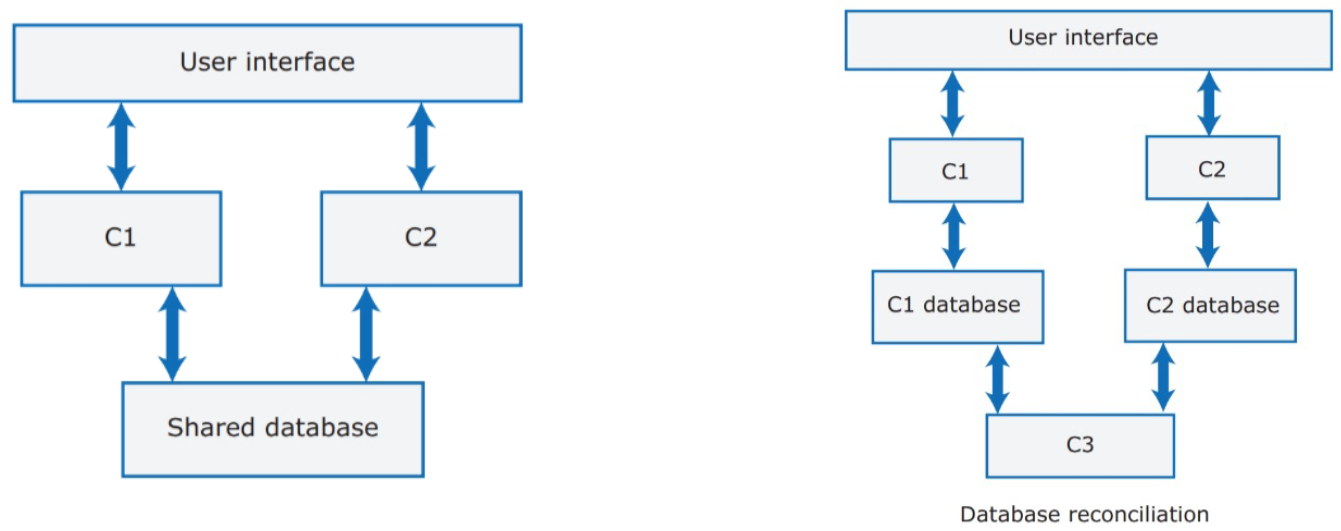
\includegraphics[width=0.90\linewidth,height=0.45\textheight,keepaspectratio]{images/04-architettura_fig4-2_partizionamento-db.png}
\caption{Partizionamento del database.}
\end{figure}

Il prezzo da pagare è la \textbf{consistenza finale} (\emph{eventual
consistency}): se il componente C1 fa una modifica (vedi Fig. 4.2),
prima o poi quella modifica deve arrivare anche al database di C3, e
questo è un costo in più. Lo stesso vale per la disponibilità: per
averne di più si possono usare più database, ma poi vanno sincronizzati.
Quando qualcosa va storto in un sistema distribuito è difficile
annullare (\emph{rollback}) le transazioni: per questo di solito
\textbf{si rinuncia alla consistenza per ottenere disponibilità}.

\begin{boxtip}{Collegamento: teorema CAP}

È lo stesso compromesso descritto dal \textbf{teorema CAP}: in presenza
di partizioni di rete un sistema distribuito non può garantire insieme
consistenza e disponibilità, quindi deve sceglierne una.

\end{boxtip}

\section{Decomposizione del sistema}\label{decomposizione-del-sistema}

Ricapitolando i termini:

\begin{itemize}
\tightlist
\item
  un \textbf{servizio} è un'unità coerente di funzionalità;
\item
  un \textbf{componente} è un'unità software che offre uno o più
  servizi;
\item
  un \textbf{modulo} è un insieme di componenti.
\end{itemize}

\begin{figure}[H]
\centering
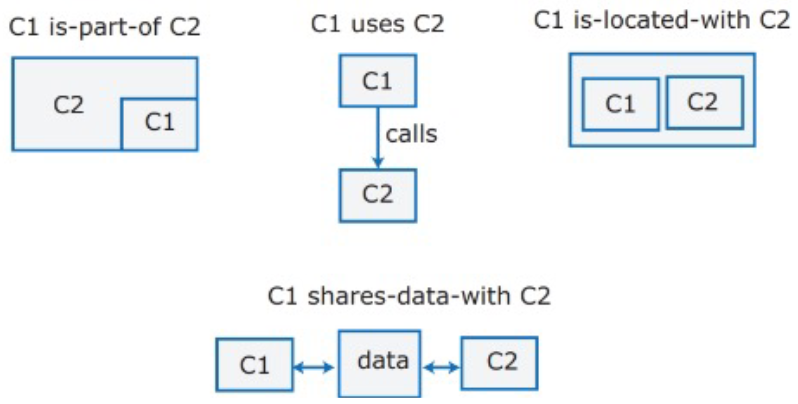
\includegraphics[width=0.70\linewidth,height=0.45\textheight,keepaspectratio]{images/04-architettura_fig4-3_relazioni-componenti.png}
\caption{Esempi di relazioni tra componenti.}
\end{figure}

Quando i componenti aumentano, le relazioni tra loro aumentano ancora
più in fretta. Per questo bisogna decomporre \textbf{quanto serve, non
di più}.

Si decompone per avere parti più semplici, da mantenere separatamente.
Una buona guida è la \textbf{separazione delle responsabilità}
(\emph{separation of concerns}): lo vedremo con i microservizi, ognuno
dei quali implementa una sola funzionalità di business. Si vogliono
anche \textbf{interfacce stabili}, da cambiare solo se davvero
necessario. Il principio ``\textbf{implementa una volta sola}'' è in
contrasto con l'idea di team indipendenti che lavorano su sistemi
indipendenti: non ci sono regole fisse, bisogna sempre trovare un
compromesso.

\begin{figure}[H]
\centering
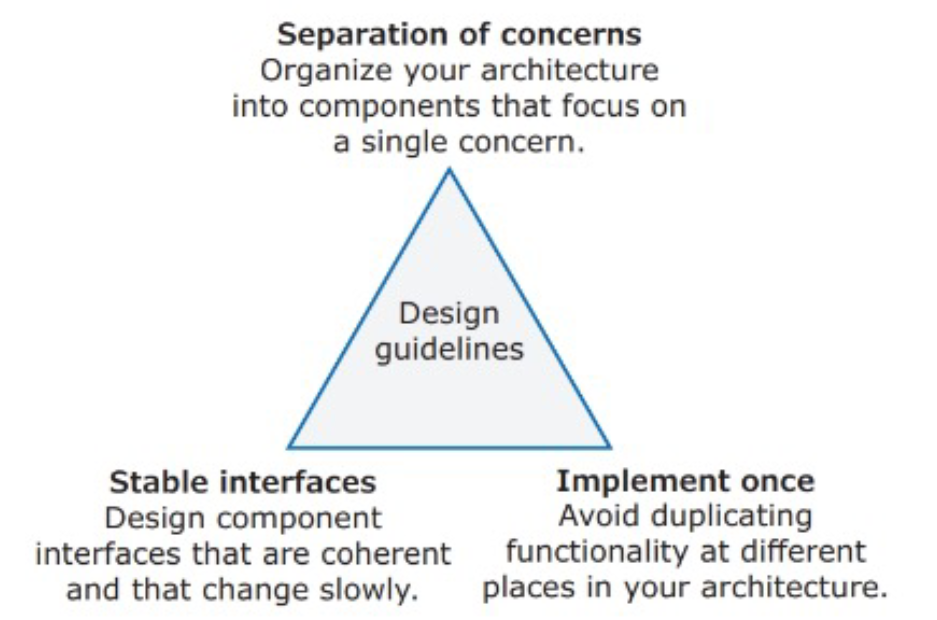
\includegraphics[width=0.70\linewidth,height=0.45\textheight,keepaspectratio]{images/04-architettura_fig4-4_linee-guida.png}
\caption{Linee guida di design per controllare la complessità.}
\end{figure}

\subsection{Architettura a livelli}\label{architettura-a-livelli}

Un altro aspetto della decomposizione è l'\textbf{architettura a
livelli} (\emph{layered architecture}). Ogni livello è un'area di
responsabilità e si considera separatamente dagli altri. Dentro ogni
livello i componenti sono indipendenti e non si sovrappongono nelle
funzionalità. Il modello architetturale è di alto livello e \textbf{non
contiene dettagli implementativi}. Di solito gli architetti partono da
livelli generici e li adattano, aggiungendone o togliendone, finché
l'architettura non va bene per i suoi obiettivi.

\begin{figure}[H]
\centering
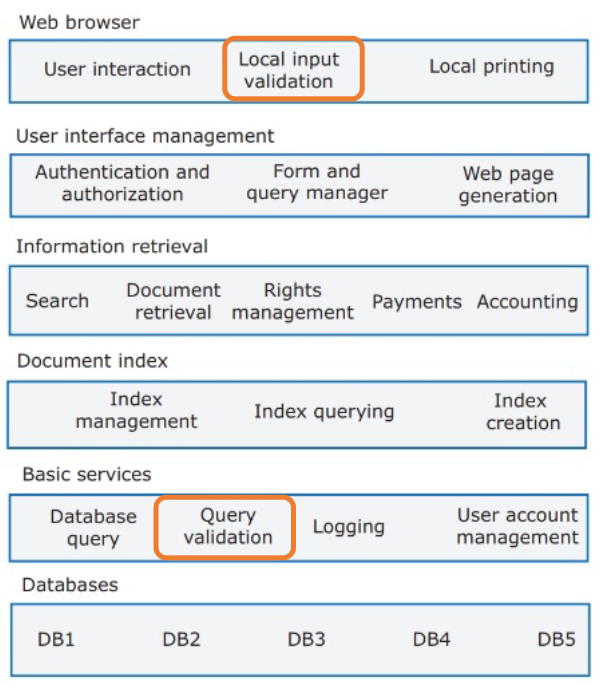
\includegraphics[width=0.70\linewidth,height=0.45\textheight,keepaspectratio]{images/04-architettura_fig4-5_architettura-a-livelli.png}
\caption{Esempio di architettura a livelli.}
\end{figure}

Alcune questioni riguardano l'intero sistema, quindi ogni livello deve
tenerne conto. Queste \textbf{cross-cutting concerns} (sicurezza,
prestazioni, affidabilità, validazione, \ldots) creano interazioni tra i
livelli. Nell'esempio di Fig. 4.5 la validazione compare in più livelli.

\begin{boxwarning}{Il dilemma dell'implementazione}

Quando si progetta l'architettura non si vuole parlare di
implementazione, per non vincolare il design con dettagli tecnici. Però
bisogna anche pensare alle possibili implementazioni per capire come
progettare: ad esempio, scegliere un database relazionale influenza i
componenti dei livelli superiori.

\end{boxwarning}

\section{Architettura di
distribuzione}\label{architettura-di-distribuzione}

\begin{boxdefinition}{Architettura di distribuzione}

L'\textbf{architettura di distribuzione} definisce i server e come i
componenti vengono assegnati ai server, cioè dove il software sarà
installato ed eseguito in produzione.

\end{boxdefinition}

Il tipo più comune è l'\textbf{architettura client-server}, adatta alle
applicazioni in cui i client accedono a un database condiviso ed
eseguono logica di business su quei dati. I client interagiscono con dei
\textbf{load balancer} (bilanciatori di carico), installati su un
cluster di server.

\begin{figure}[H]
\centering
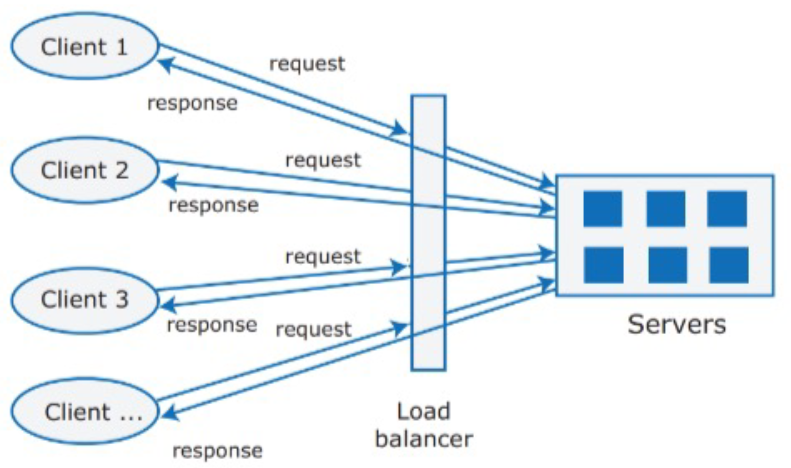
\includegraphics[width=0.70\linewidth,height=0.45\textheight,keepaspectratio]{images/04-architettura_fig4-6_client-server.png}
\caption{Esempio di architettura client-server.}
\end{figure}

Un pattern molto usato è il \textbf{Model-View-Controller (MVC)}, che
struttura il codice dividendolo in tre parti: \textbf{Model},
\textbf{View} e \textbf{Controller}. In molti casi aiuta anche a capire
come implementare la comunicazione tra le parti, e questo influisce
sulla semplicità ed efficienza dell'architettura (spesso la
comunicazione avviene con \textbf{HTTP + JSON}).

\begin{figure}[H]
\centering
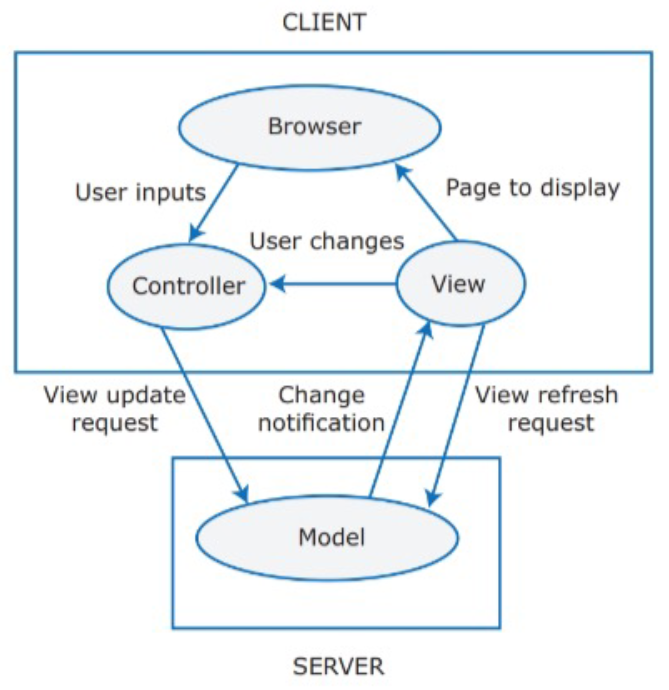
\includegraphics[width=0.45\linewidth,height=0.45\textheight,keepaspectratio]{images/04-architettura_fig4-7_mvc.png}
\caption{Model-View-Controller.}
\end{figure}

Il pattern di Fig. 4.7 \textbf{separa la logica di presentazione dei
dati dalla logica di business}. Si colloca al livello logico/di business
e si usa nelle architetture multi-tier.

\begin{figure}[H]
\centering
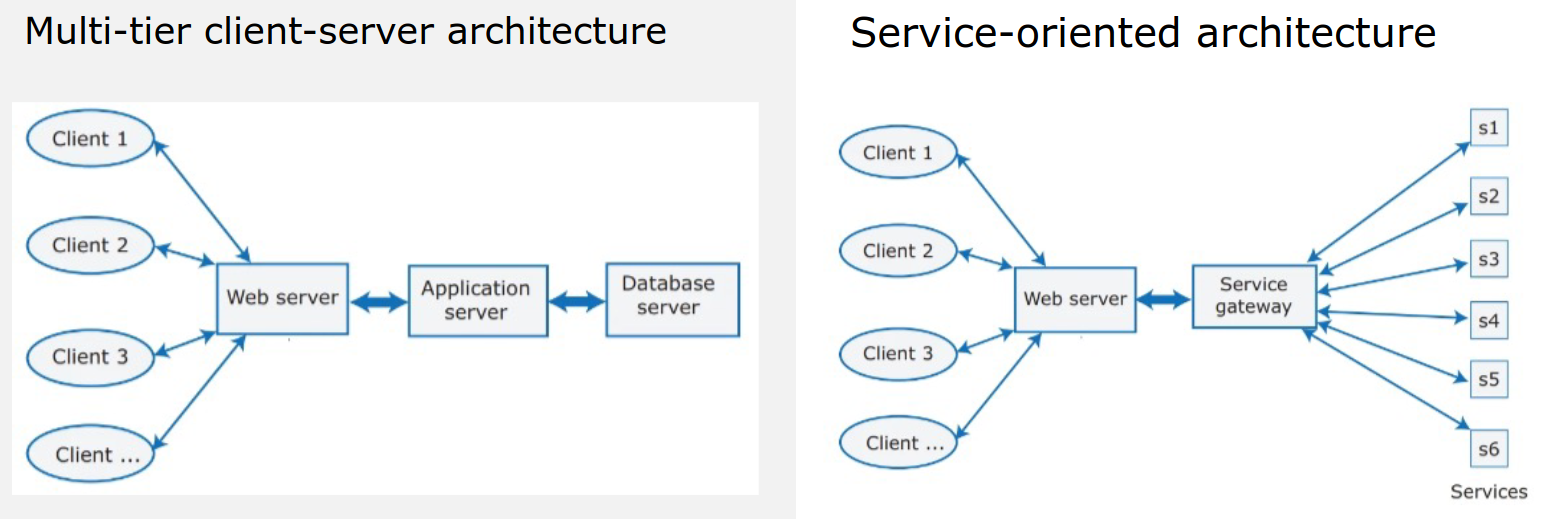
\includegraphics[width=1.00\linewidth,height=0.45\textheight,keepaspectratio]{images/04-architettura_fig4-8_tipi-client-server.png}
\caption{Tipi comuni di architettura client-server.}
\end{figure}

L'architettura client-server si può realizzare in vari modi (Fig. 4.8).
L'\textbf{architettura orientata ai servizi} (\emph{Service-Oriented
Architecture}, SOA) è leggermente diversa: ha un \textbf{service
gateway} che smista le richieste al servizio giusto.

La scelta dell'architettura di distribuzione dipende da:

\begin{itemize}
\tightlist
\item
  \textbf{Tipo di dati e aggiornamenti}: se si usano soprattutto dati
  strutturati modificati da più feature, di solito conviene un
  \textbf{unico database condiviso} che gestisca lock e transazioni. Se
  i dati sono distribuiti tra i servizi, serve un modo per tenerli
  consistenti, e questo appesantisce il sistema.
\item
  \textbf{Piattaforma di esecuzione}: se il sistema girerà nel cloud con
  utenti che accedono via Internet, di solito conviene
  un'\textbf{architettura a servizi}, perché scalare è più semplice. Se
  è un sistema aziendale che gira su server locali, può andare meglio
  un'architettura \textbf{multi-tier}.
\item
  \textbf{Frequenza dei cambiamenti}: se si prevede che alcuni
  componenti vengano cambiati o sostituiti spesso, isolarli come servizi
  separati (dentro container) rende i cambiamenti più semplici.
\end{itemize}

\section{Scelte tecnologiche}\label{scelte-tecnologiche}

Alcune scelte tecnologiche sono particolarmente importanti, perché se il
design del prodotto cambia bisogna cambiare anche loro, con più
complessità e costi durante lo sviluppo. Le principali sono:

\begin{itemize}
\tightlist
\item
  \textbf{Database}: si può scegliere un database relazionale
  \textbf{SQL} (dati organizzati in tabelle strutturate: adatto quando
  servono le transazioni e le strutture dati sono prevedibili e
  semplici) oppure un database non strutturato \textbf{NoSQL}
  (organizzazione dei dati più flessibile e definita dall'utente, anche
  gerarchica: più efficiente per l'analisi dei dati e per l'elaborazione
  concorrente di ``big data'').
\item
  \textbf{Piattaforma di rilascio} (\emph{delivery platform}): dove
  girerà il prodotto, web o mobile. Ogni piattaforma ha i suoi problemi
  (sul mobile: connessione intermittente, potenza del processore,
  gestione della batteria, schermo piccolo, tastiera a schermo).
  Conviene decidere presto per iniziare prima lo sviluppo.
\item
  \textbf{Server}: il prodotto girerà in un cloud pubblico o su server
  interni? La maggior parte dei prodotti consumer usa
  \textbf{microservizi} in container, installati nel cloud (architettura
  SOA). I prodotti aziendali invece si preoccupano di più della
  sicurezza nel cloud (dove e come vengono salvati i dati dei clienti).
  Deciso di andare nel cloud, bisogna scegliere il provider: attenzione,
  poi è difficile spostarsi da un provider all'altro (\textbf{vendor
  lock-in}).
\item
  \textbf{Open source}: esistono componenti open source adatti da
  integrare nel prodotto? Sono abbastanza sicuri?
\item
  \textbf{Strumenti di sviluppo}: le tecnologie di sviluppo (toolkit
  mobile, framework web, \ldots) influenzano l'architettura. Anche le
  tecnologie che gli sviluppatori conoscono già finiscono per
  influenzarla indirettamente.
\end{itemize}

\section{Enterprise Application
Integration}\label{enterprise-application-integration}

Le \textbf{applicazioni enterprise} sono grandi sistemi software pensati
per lavorare in un'organizzazione (aziende, pubblica amministrazione).
L'utente vede solo il front-end, ma dietro c'è molta funzionalità di
back-end fatta di tanti servizi. Questi servizi eterogenei si possono
classificare come:

\begin{itemize}
\tightlist
\item
  \textbf{source}: servizi che fanno solo richieste;
\item
  \textbf{sink}: servizi che rispondono solo alle richieste;
\item
  un misto dei due.
\end{itemize}

I servizi comunicano con tipi di dati eterogenei (con rappresentazioni
diverse anche per dati simili), e queste informazioni possono essere
condivise via rete con altre organizzazioni. Tutta questa complessità fa
delle applicazioni enterprise delle \textbf{applicazioni distribuite
multi-servizio}, i cui servizi devono lavorare insieme ed essere
integrati in modo adeguato.

La domanda architetturale è: come integrare tutto in modo
\textbf{coerente, estendibile e manutenibile}? Un modo per gestire la
complessità è usare i \textbf{pattern}.

\begin{boxdefinition}{Pattern}

Un \textbf{pattern} è un'astrazione di alto livello di una soluzione
accettata e riusabile per un problema ricorrente. Si descrive con:

\begin{itemize}
\tightlist
\item
  \textbf{problema}: quale problema risolve;
\item
  \textbf{contesto}: in quale situazione (per lo stesso problema possono
  esistere pattern diversi);
\item
  \textbf{forze}: perché conviene usare il pattern per quel problema;
\item
  \textbf{soluzione}: come applicare il pattern.
\end{itemize}

\end{boxdefinition}

L'idea dei pattern è non reinventare la ruota e usare soluzioni già
consolidate. L'\textbf{Enterprise Application Integration (EAI)} è
un'astrazione riusabile di soluzioni collaudate per i problemi tipici
che nascono quando si integrano i componenti e i servizi di
un'applicazione enterprise.

\subsection{Pattern}\label{pattern}

Questi pattern sono stati studiati più di 20 anni fa. Tra tutti, i più
usati sono i \textbf{pattern di messaggistica} (\emph{messaging
patterns}), mostrati in Fig. 4.9 (catalogo completo su
\href{https://www.enterpriseintegrationpatterns.com/patterns/messaging/}{enterpriseintegrationpatterns.com}).

\begin{figure}[H]
\centering
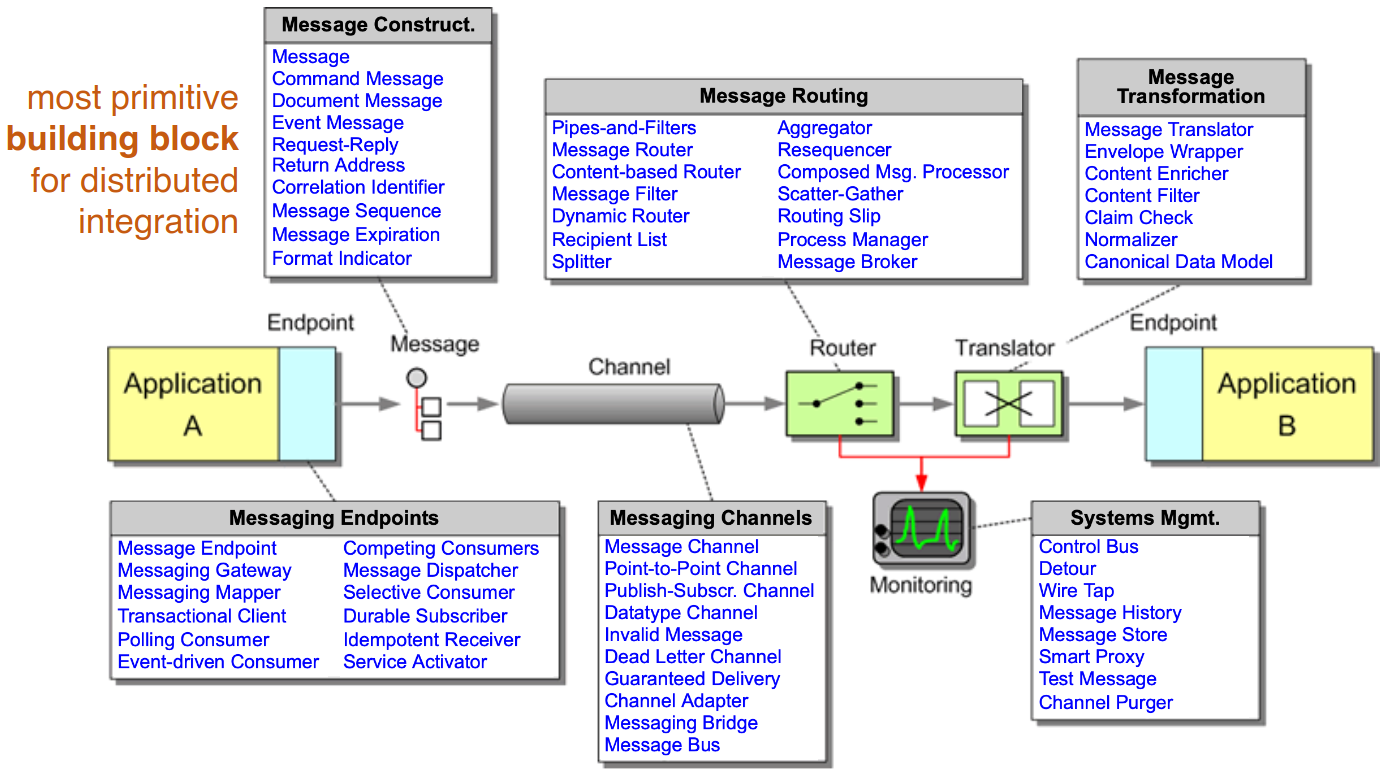
\includegraphics[width=1.00\linewidth,height=0.45\textheight,keepaspectratio]{images/04-architettura_fig4-9_messaging-patterns.png}
\caption{I pattern di messaggistica.}
\end{figure}

\begin{boxdefinition}{Messaggio}

Un \textbf{messaggio} è un pezzo di dati discreto inviato da un servizio
a un altro. Di solito è formato da un \textbf{header} (metadati) e un
\textbf{body} (il contenuto, \emph{payload}).

\end{boxdefinition}

Esempi concreti sono i \textbf{document message} (solo dati), gli
\textbf{event message} (notifiche di eventi) e i \textbf{command
message} (comandi per eseguire un'azione).

\begin{figure}[H]
\centering
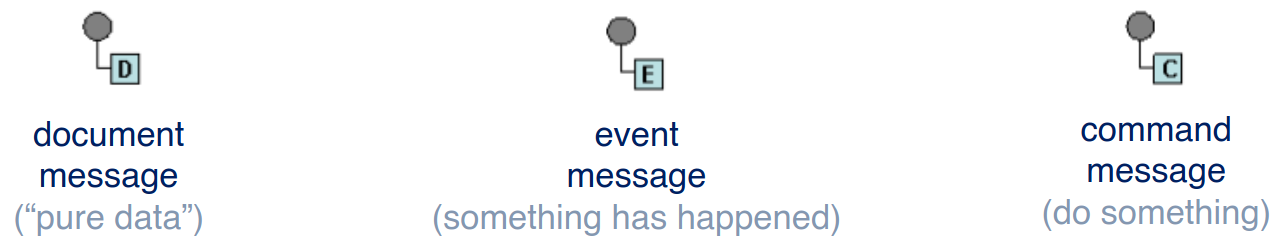
\includegraphics[width=1.00\linewidth,height=0.45\textheight,keepaspectratio]{images/04-architettura_fig4-10_tipi-messaggi.png}
\caption{Esempi di messaggi concreti.}
\end{figure}

Scambiandosi messaggi, i servizi non sono legati strettamente tra loro:
la comunicazione a messaggi permette l'\textbf{accoppiamento debole}
(\emph{loose coupling}). Si realizza con i \textbf{canali}
(\emph{channel}): astrazioni che portano i messaggi da una sorgente a
una destinazione (implementate in vari modi: RPC, HTTP, TCP, \ldots). I
canali sono \textbf{a senso unico}, quindi la comunicazione è
naturalmente \textbf{asincrona}; una comunicazione sincrona
(richiesta/risposta) usa due canali.

I servizi applicativi di solito sono indipendenti dal sistema di
messaggistica, quindi si usano degli \textbf{adapter} per mandare sui
canali i dati specifici dell'applicazione. I \textbf{message endpoint}
permettono ai servizi di inviare e ricevere messaggi dai canali.
Esistono vari tipi di canale:

\begin{itemize}
\tightlist
\item
  \textbf{point-to-point}: garantisce che un messaggio venga ricevuto da
  \textbf{un solo} destinatario (è quello di Fig. 4.11);
\item
  \textbf{publish-subscribe}: il publisher consegna una copia di ogni
  messaggio a \textbf{ogni} subscriber.
\end{itemize}

\begin{figure}[H]
\centering
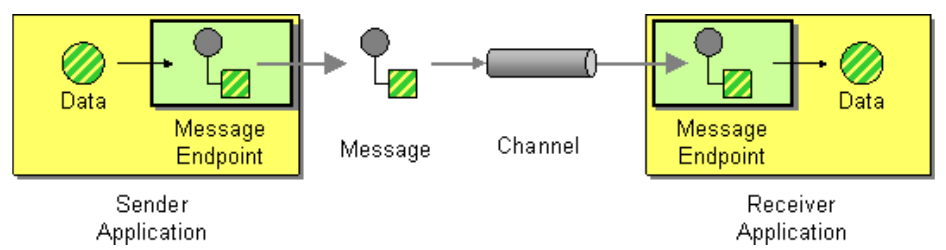
\includegraphics[width=1.00\linewidth,height=0.45\textheight,keepaspectratio]{images/04-architettura_fig4-11_canale-messaggi.png}
\caption{Integrazione semplice con comunicazione a messaggi.}
\end{figure}

Questo da solo però non basta: cosa succede se il servizio che riceve si
aspetta un formato di dati diverso? Un \textbf{message translator}
adatta il messaggio al servizio destinatario. Possono servire anche
altri passaggi, ad esempio decidere come instradare i messaggi verso
destinazioni diverse o multiple, come dividerli e come aggregarli.

\subsection{Pipes and Filters}\label{pipes-and-filters}

Lo stile architetturale \textbf{pipes and filters} (insieme agli altri
pattern EIP) permette di strutturare le integrazioni più complesse. I
messaggi attraversano più passi di elaborazione (i \textbf{filter}), e
ogni componente invia i messaggi lungo i canali (le \textbf{pipe}) a cui
è collegato. I messaggi scorrono nelle pipe e, quando arrivano a un
filter, possono essere trasformati prima di raggiungere il \textbf{sink}
(la destinazione finale).

\begin{boxexample}{Loan Broker}

Un esempio classico di EAI è il \textbf{Loan Broker}: arriva una
richiesta di prestito, il \textbf{Credit Bureau} la valuta (punteggio di
credito), la \textbf{Rule Base} decide a quali banche inoltrarla, le
\textbf{banche} accettano o rifiutano il prestito. Tutte le risposte
vengono aggregate e rimandate a chi ha fatto la richiesta. L'area grigia
in figura rappresenta il servizio di prestito.

\end{boxexample}

\begin{figure}[H]
\centering
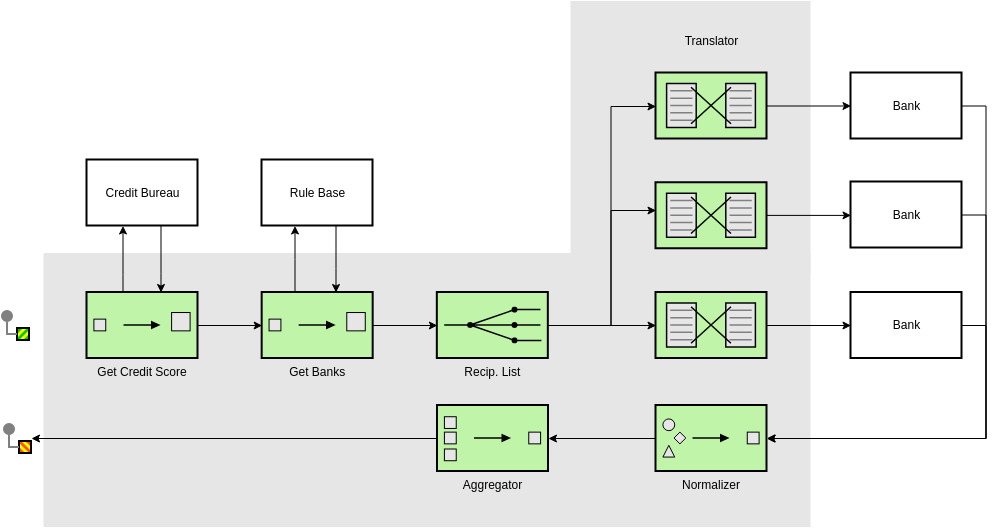
\includegraphics[width=1.00\linewidth,height=0.45\textheight,keepaspectratio]{images/04-architettura_fig4-12_loan-broker.png}
\caption{Il design del Loan Broker.}
\end{figure}

Altri pattern usati nell'esempio:

\begin{itemize}
\tightlist
\item
  \textbf{Content Enricher}: usa informazioni del messaggio in arrivo
  (es. campi chiave) per recuperare dati da una fonte esterna e li
  aggiunge al messaggio. Le informazioni originali si possono tenere o
  scartare. In Fig. 4.12 le chiamate \emph{Get Credit Score} e \emph{Get
  Banks} sono esempi di arricchimento.
\item
  \textbf{Router}: ci sono due categorie principali. I
  \textbf{content-based router} instradano in base al tipo di messaggio
  (nell'header) o al suo contenuto (nel body). I \textbf{context-based
  router} instradano in base a informazioni di contesto prese da una
  configurazione centrale. In generale un message router è collegato a
  più canali e contiene la logica per decidere su quale inviare.
\end{itemize}

\begin{figure}[H]
\centering
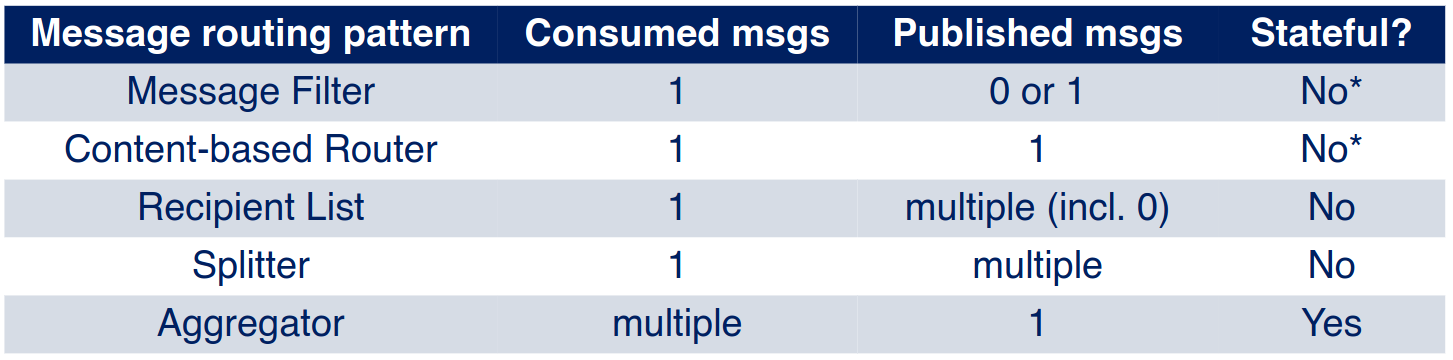
\includegraphics[width=1.00\linewidth,height=0.45\textheight,keepaspectratio]{images/04-architettura_fig4-13_routing-pattern.png}
\caption{Pattern di routing dei messaggi.}
\end{figure}

Una \textbf{recipient list} esamina il messaggio in arrivo, decide la
lista dei destinatari e lo inoltra su tutti i canali associati a quei
destinatari. Un \textbf{content-based router} invia ogni messaggio al
destinatario giusto in base al suo contenuto.

\begin{itemize}
\tightlist
\item
  \textbf{Normalizer}: traduce i messaggi in un \textbf{formato di dati
  comune}. Di solito si realizza combinando più pattern: si possono
  comporre pattern per crearne di composti, come nel caso del
  normalizer.
\end{itemize}

\begin{figure}[H]
\centering
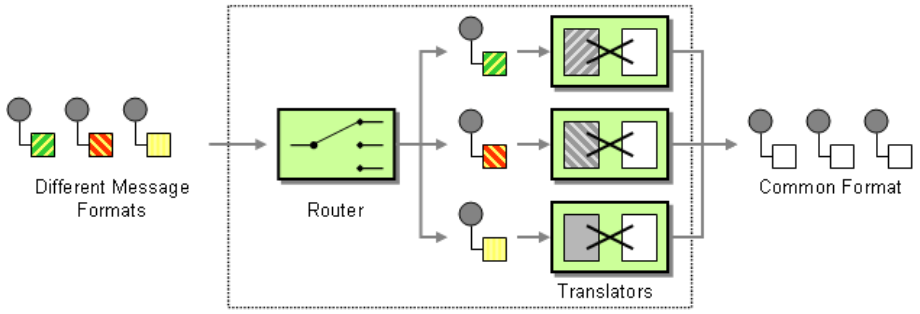
\includegraphics[width=0.90\linewidth,height=0.45\textheight,keepaspectratio]{images/04-architettura_fig4-14_normalizer.png}
\caption{Schema del Normalizer.}
\end{figure}

\begin{itemize}
\tightlist
\item
  \textbf{Aggregator}: un aggregator (\textbf{con stato}) raccoglie e
  memorizza i singoli messaggi finché non ha ricevuto un insieme
  completo di messaggi collegati (vedi Fig. 4.13). Si usa quando alcuni
  passi dell'integrazione possono avvenire \textbf{in parallelo}:
  processi indipendenti girano in parallelo e i loro risultati vengono
  aggregati per decidere come proseguire.
\end{itemize}
